\chapter{Project Documentation}
% --------------------------------------%
\section{Project Plan}
\subsection{Project Overview}
The goal of this project is to create and organize a lab, which shows and explains future students of the Ostschweizer Fachhochschule (OST) how reverse engineering is performed and which tactics are used to get information out of a program. To accomplish this task, the lab will have several exercises organized in the different domains. These exercises will be accessible through the Hacking-Lab hosted on the OST server. 

\subsubsection*{Hand-In}
The finished Report will be hended in according to the rules set by the "Studiengangsleitung Informatik" and the supervisor:
\begin{itemize}
    \item 2 PDF will be handed in. One for the supervisor and one for the archive.
    \item 1 printed version will be handed in to the supervisor for reading and grading.
\end{itemize}

\subsection{Management}
\subsubsection*{Time Management}
The project started on the first week of the semester (KW 38) and ends in week 51 giving us around 14 weeks to be done with the Hand-In. \\
Since the module has a total ECTS of 8 each of the students has to work around 240h during the semester which can be seen in table \ref{time_ects} together with the total planned time investment. This means, that per week each student should work around 17.1 hours.

\begin{table}
    \centering
    \begin{tabular}{||c c c c||} 
        \hline
        Name & ECTS & Time spent per Week [h] & Total Time spent [h]\\ [0.5ex] 
        \hline\hline
        Gianluca Nenz & 8 & 17.1 & 240 \\ 
        \hline
        Ronny Mueller & 8 & 17.1 & 240 \\
        \hline
        Thomas Kleb & 8 & 17.1 & 240 \\ 
        \hline
        \textbf{Total} & 32 & 52.3 & 720 \\[1ex] 
        \hline
    \end{tabular}
    \caption{Time Investments}
    \label{time_ects}
\end{table}

\subsubsection*{Planning}
In the past modules Software Engineering Practices 1 and 2 (SEP 1 + 2) we were introduced to different ways to plan and organize a project. The main tools we learned, RUP (Rational Unified Process) and Scrum, are mainly used in software development but can be adapted to other projects aswell. They both use different aspects of time management and organisation which is why we intend to apply them to our project.

\subsubsection*{\textit{RUP (Rational Unified Process)}}
\label{rup_section}
RUP is a process which allows a team to distribute a longterm plan over a given time and section it into multiple steps and parts. RUP has four main phases which have characteristics to be taken care of: \\

\vspace{0.2cm}

\noindent \textbf{Inception:} The goal in this phase is to propose the project, identifying the criterias to be assessed and a first estimation of risk and success. This part should take less than 5\% of the total time.\\
\textbf{Elaboration:} The elaboration phase is used to identify the requirements and the architecture. It should also be used to get rid or at least plan for the highest risks. After this phase the team has a plan of what to work on and how much work is to be done. This part should take about 25\% of the total time. \\
\textbf{Construction:} This step is where the team implements the functionality of the product and starts working on the development. A big part of it, is to get rid of risks which hinder the process. This is the biggest part, taking about 50\% of the total time.\\
\textbf{Transition:} This final step of RUP is ued to test the product and finalize the deployment. About 20\% of the time should be planned for it.\\

\pagebreak
\subsubsection*{\textit{Scrum}}
\label{scrum_section}
Scrum is a framework that helps teams work together. It is most frequently used by software development teams but its principles and lessons can be applied to all kinds of teamwork. It helps teams to find solutions for complex problems with the help of planning. It consists of different roles and parts to make it work:

\begin{multicols}{2}
    \begin{itemize}
        \item Scrum Team
        \begin{itemize}
            \item Developers
            \item Product Owner
            \item Scrum Master
        \end{itemize}
    \end{itemize}
    \begin{itemize}
        \item Scrum Events
        \begin{itemize}
            \item The Sprint
            \item Sprint Planning
            \item Daily Scrum
            \item Sprint Review
            \item Sprint Retrospective
        \end{itemize}
    \end{itemize}
    \columnbreak
    \begin{itemize}
        \item Scrum Artifacts
        \begin{itemize}
            \item Product Backlog
            \item Print Backlog
            \item Increment
        \end{itemize}
    \end{itemize}
    \begin{itemize}
        \item Scrum Values
        \begin{itemize}
            \item Commitment
            \item Focus
            \item Openness
            \item Respect
            \item Courage
        \end{itemize}
    \end{itemize}
\end{multicols}

\begin{figure}[h]
    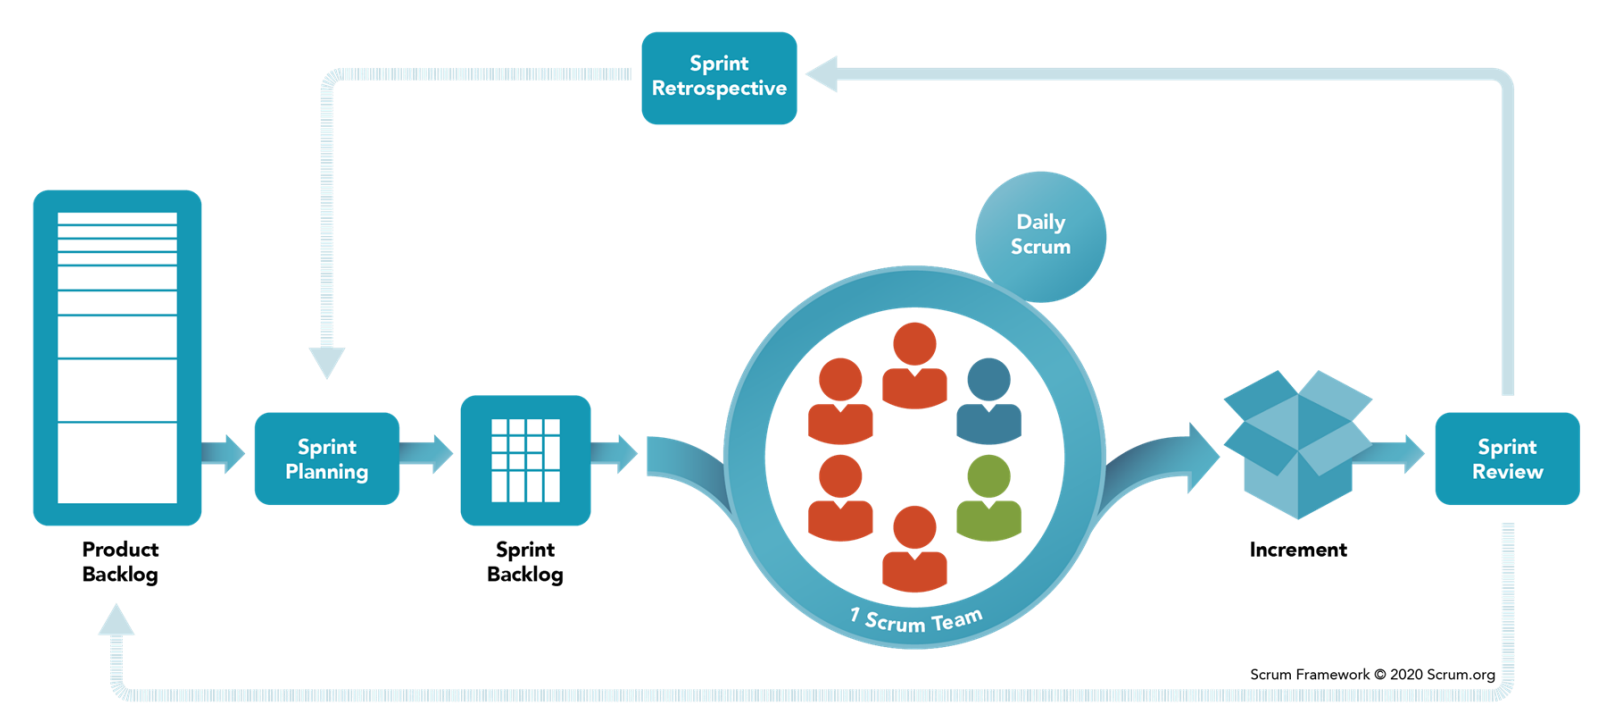
\includegraphics[width=\linewidth]{04_Project-Documentation/scrum.png}
    \caption{Scrum}
    \label{scrum_img}
\end{figure}
\subsection{Organisation}

\subsubsection*{Participants}
The "Studienarbeit"-Team consists of three students: Gianluca Nenz, Ronny Muel\-ler and Thomas Kleb. Work on the project and documentation will be evenly distributed between these three participants. Bigger decisions are made as a team in either the meetings with or without the advisor (the advisor will be notified on anyone made).

\subsubsection*{Advisor}
The teams advisor for the "Studienarbeit" is Ivan Buetler who is teaching cyber security modules at the OST.

\subsubsection*{Division of Labor}
The project has multiple facets that need to be taken care of. This is why the team has decided to distributed the work load between the three. This doesn't mean that the work is done by only the chosen student but rather that he is the one responsible that it works as planned.
\begin{table}[H]
    \begin{tabular}[t]{||p{4cm}||}
        \hline
        Gianluca Nenz \\
        \hline\hline
        Work 1 \\ 
        \hline
        Work 2 \\
        \hline
        Work 3 \\ 
        \hline
        Work 4\\[1ex] 
        \hline
    \end{tabular}
    \hfill
    \begin{tabular}[t]{||p{4cm}||}
        \hline
        Ronny Mueller \\
        \hline\hline
        Work 1 \\ 
        \hline
        Work 2 \\
        \hline
        Work 3 \\ 
        \hline
        Work 4\\[1ex] 
        \hline
    \end{tabular}
    \hfill
    \begin{tabular}[t]{||p{4cm}||}
        \hline
        Thomas Kleb \\
        \hline\hline
        Work 1 \\ 
        \hline
        Work 2 \\
        \hline
        Work 3 \\ 
        \hline
        Work 4\\[1ex] 
        \hline
    \end{tabular}
    \caption{Work Distribution per Student}
    \label{work_dis}
\end{table}

\subsection{Planning and Milestones}

\subsubsection*{Phases and Iterations}
The project is comprised of the four steps explained in \nameref{rup_section}. Each of those phases has multiple iterations which create the different sprints for the project. The meetings with the advisor will be on thursdays while the team meetings will be held tuesdays. Each iteration / sprint will be of a seven day length. \\

\noindent We started the "Studienarbeit" before we began with the regular school. In the week before we each made research and plans about the comming project. After having a talk with the advisor it was decided to first find out the level of knowledge each student has to make it easier for the advisor to plan.
\begin{table}[H]
    \centering
    \begin{tabular}{|p{0.1\linewidth}|p{0.15\linewidth}|p{0.15\linewidth}|p{0.46\linewidth}|}
        \hline
        \multicolumn{4}{||c||}{\textbf{Inception}} \\
        \hline \hline
        Iteration & Start & End & Description \\
        \hline \hline
        0 & 12.09.2022 & 18.09.2022 & Collection of Ideas and planning first meeting\\
        \hline
        1 & 19.09.2022 & 25.09.2022 & First meeting and handout of exercises to assess the knowledge of the students \\
        \hline
        2 & 26.09.2022 & 02.10.2022 & Working on the exercises and receiving solutions for harder ones \\
        \hline
    \end{tabular}
    \caption{RUP: Inception Phase Planning}
    \label{inception_table}
\end{table}

\noindent The elaboration phase is used to plan and assess the possible risks in this project. This consists of a documentation structure, the project plan and the risk management to make sure the construction phase has no major hickups.
\begin{table}[H]
    \centering
    \begin{tabular}{|p{0.1\linewidth}|p{0.15\linewidth}|p{0.15\linewidth}|p{0.46\linewidth}|}
        \hline
        \multicolumn{4}{||c||}{\textbf{Elaboration}} \\
        \hline \hline
        Iteration & Start & End & Description \\
        \hline \hline
        3 & 03.10.2022 & 09.10.2022 &  First big meeting with advisor; Creating project plan and risk analysis.\\
        \hline
        4 & 10.10.2022 & 16.10.2022 & ---- \\
        \hline
        5 & 17.10.2022 & 23.10.2022 & ---- \\
        \hline
    \end{tabular}
    \caption{RUP: Elaboration Phase Planning}
    \label{elaboration_table}
\end{table}

\noindent The construction phase is where the labs are primarily built. 
\begin{table}[H]
    \centering
    \begin{tabular}{|p{0.1\linewidth}|p{0.15\linewidth}|p{0.15\linewidth}|p{0.46\linewidth}|}
        \hline
        \multicolumn{4}{||c||}{\textbf{Construction}} \\
        \hline \hline
        Iteration & Start & End & Description \\
        \hline \hline
        6 & 24.10.2022 & 30.10.2022 & ----\\
        \hline
        7 & 31.10.2022 & 06.11.2022 & ---- \\
        \hline
        8 & 07.11.2022 & 13.11.2022 & ---- \\
        \hline
        9 & 14.11.2022 & 20.11.2022 & ---- \\
        \hline
        10 & 21.11.2022 & 27.11.2022 & ---- \\
        \hline
        11 & 28.11.2022 & 04.12.2022 & ---- \\
        \hline
    \end{tabular}
    \caption{RUP: Construction Phase Planning}
    \label{construction_table}
\end{table}

\noindent To make sure enough time is planned a buffer week was added to the transition phase. This phase is also mainly used to finish up the documentation and implement the different labs to Hacking Lab. The last week is used to clean up and hand in the documentation and abstract to both the OST and the advisor.
\begin{table}[H]
    \centering
    \begin{tabular}{|p{0.1\linewidth}|p{0.15\linewidth}|p{0.15\linewidth}|p{0.46\linewidth}|}
        \hline
        \multicolumn{4}{||c||}{\textbf{Transition}} \\
        \hline \hline
        Iteration & Start & End & Description \\
        \hline \hline
        12 & 05.12.2022 & 11.12.2022 & Buffer \\
        \hline
        13 & 12.12.2022 & 18.12.2022 & ---- \\
        \hline
        14 & 19.12.2022 & 23.12.2022 & ---- \\
        \hline
    \end{tabular}
    \caption{RUP: Transition Phase Planning}
    \label{transition_table}
\end{table}

\subsubsection*{Milestones}
To guarantee the success of the project milestones were defined with a deadline.

\begin{table}[H]
    \centering
    \begin{tabular}[]{|| p{5cm} | c | p{6.2cm} ||}
        \hline
        Milestones & Deadline & Description \\
        \hline \hline
        M1 - Solving RE Exercises & 05.10.2022 & The Team solves the given exercises to find the level of RE knowledge. \\
        \hline
        M2 - Defining Problem Domains and Learnconcepts& ---- & ---- \\
        \hline
        M3 - Lab Concepts & ---- & ---- \\
        \hline
        M4 - Refining Labs & ---- & ---- \\
        \hline
        M5 - Setup Labs& ---- & ---- \\
        \hline
        M6 - Hand-In& ---- & ---- \\
        \hline
    \end{tabular}
\end{table}

\subsubsection*{Time Tracking}
For time tracking the team has decided on using GitLabs integrated time tracking. 
\subsubsection*{Issue Tracking}

\subsubsection*{Meetings}
The team has meetings each tuesday to elaborate problems and check up on the progress. This meetings are also used to distributed the work load and the different parts of the sprint. \\
On Thursdays the team meets the advisor Ivan Buetler to inform him on the progress done and the problems that came up. These meetings have different time schedules to fit everyones calender. \\
Each meeting will be documented and uploaded to the GIT repository. After each meeting the participants should know what to do and how to contact each other if any problems arise.
\subsubsection*{CI/CD}

\subsubsection*{Testing}

\subsubsection*{Projectmanagment}
The whole project will use a GitLab repository. To make sure no confusion happens a multirepo principle is used where one repository is for the documentation and protocols only and other are for code, information gathered, etc. Each student works on a branch and before pushing to the main branch has another student look into the code / text written. 
% --------------------------------------%
\section{Risk Analysis}

\section{Project Monitoring}

\subsubsection*{Overview}

\subsubsection*{Milestones}

\subsubsection*{Time Tracking}

% --------------------------------------%
\section{Personal Rapports}

\subsubsection*{Gianluca Nenz}

\subsubsection*{Ronny Mueller}

\subsubsection*{Thomas Kleb}